
\section{Übertragungsleitungen II}
\label{section:uebertragungsleitungen_2}
\begin{frame}%STARTCONTENT

\frametitle{Wellenwiderstand}
\begin{itemize}
  \item Unabhängig von der Länge der Leitung
  \item Unabhängig von den an die Leitung angeschlossenen Geräten
  \item Abhängig vom Querschnittsaufbau (Leiter, ggf. Dielektrikum)
  \item Im Bereich der Hochfrequenz ist der Wellenwiderstand weitgehend konstant
  \end{itemize}
\end{frame}

\begin{frame}
\only<1>{
\begin{QQuestion}{EG301}{Der Wellenwiderstand einer Leitung~...}{ist im HF-Bereich in etwa konstant und unabhängig vom Leitungsabschluss.}
{ist völlig frequenzunabhängig.}
{hängt von der Beschaltung am Leitungsende ab.}
{hängt von der Leitungslänge und der Beschaltung am Leitungsende ab.}
\end{QQuestion}

}
\only<2>{
\begin{QQuestion}{EG301}{Der Wellenwiderstand einer Leitung~...}{\textbf{\textcolor{DARCgreen}{ist im HF-Bereich in etwa konstant und unabhängig vom Leitungsabschluss.}}}
{ist völlig frequenzunabhängig.}
{hängt von der Beschaltung am Leitungsende ab.}
{hängt von der Leitungslänge und der Beschaltung am Leitungsende ab.}
\end{QQuestion}

}
\end{frame}

\begin{frame}
\frametitle{Leitungen}
\begin{columns}
    \begin{column}{0.48\textwidth}
    \begin{itemize}
  \item Paralleldraht-Speiseleitung
  \item Koaxialkabel
  \end{itemize}

    \end{column}
   \begin{column}{0.48\textwidth}
       \begin{itemize}
  \item Das Koaxialkabel vermeidet bei bestimmungsgemäßer Anwendung unerwünschte Abstrahlung
  \item Unerwünschte Abstrahlungen können durch \emph{Mantelwellen} auftreten
  \item Mantelwellen lassen sich durch Mantelwellensperren unterdrücken
  \end{itemize}

   \end{column}
\end{columns}

\end{frame}

\begin{frame}
\only<1>{
\begin{QQuestion}{EG302}{Welche Leitungen sollten für die HF-Verbindungen zwischen Einrichtungen in der Amateurfunkstelle verwendet werden, um unerwünschte Abstrahlungen zu vermeiden?}{Symmetrische Feederleitungen}
{Hochwertige Koaxialkabel}
{Unabgestimmte Speiseleitungen}
{Hochwertige abgeschirmte Netzanschlusskabel}
\end{QQuestion}

}
\only<2>{
\begin{QQuestion}{EG302}{Welche Leitungen sollten für die HF-Verbindungen zwischen Einrichtungen in der Amateurfunkstelle verwendet werden, um unerwünschte Abstrahlungen zu vermeiden?}{Symmetrische Feederleitungen}
{\textbf{\textcolor{DARCgreen}{Hochwertige Koaxialkabel}}}
{Unabgestimmte Speiseleitungen}
{Hochwertige abgeschirmte Netzanschlusskabel}
\end{QQuestion}

}
\end{frame}

\begin{frame}
\frametitle{Einkopplungen}
\begin{itemize}
  \item Kabel, die direkt neben Koaxialkabel verlegt werden, können Einkopplungen erfahren
  \item Dadurch gelangt Hochfrequenz beispielsweise ins Stromnetz
  \item Und Leistung zur Antenne geht verloren
  \end{itemize}
\end{frame}

\begin{frame}
\only<1>{
\begin{QQuestion}{EG306}{Um Ordnung in der Amateurfunkstelle herzustellen, verlegen Sie alle Netzanschlusskabel und HF-Speiseleitungen in einem Kabelkanal. Welchen Nachteil kann diese Maßnahme haben?}{Die nebeneinander liegenden HF- und Netzkabel können zu unerwünschter \qty{50}{\Hz}-Modulation auf dem Koaxialkabel führen.}
{Die nebeneinander liegenden HF- und Netzkabel können Einkopplungen in das Versorgungsnetz hervorrufen.}
{Zwischen den nebeneinander liegenden HF- und Netzkabeln kann es zu Spannungsüberschlägen kommen.}
{Die nebeneinander liegenden HF- und Netzkabel können sich bei guter Isolierung nicht gegenseitig beeinflussen.}
\end{QQuestion}

}
\only<2>{
\begin{QQuestion}{EG306}{Um Ordnung in der Amateurfunkstelle herzustellen, verlegen Sie alle Netzanschlusskabel und HF-Speiseleitungen in einem Kabelkanal. Welchen Nachteil kann diese Maßnahme haben?}{Die nebeneinander liegenden HF- und Netzkabel können zu unerwünschter \qty{50}{\Hz}-Modulation auf dem Koaxialkabel führen.}
{\textbf{\textcolor{DARCgreen}{Die nebeneinander liegenden HF- und Netzkabel können Einkopplungen in das Versorgungsnetz hervorrufen.}}}
{Zwischen den nebeneinander liegenden HF- und Netzkabeln kann es zu Spannungsüberschlägen kommen.}
{Die nebeneinander liegenden HF- und Netzkabel können sich bei guter Isolierung nicht gegenseitig beeinflussen.}
\end{QQuestion}

}
\end{frame}

\begin{frame}
\frametitle{Unsymmetrische Speiseleitung}
\begin{columns}
    \begin{column}{0.48\textwidth}
    
\begin{figure}
    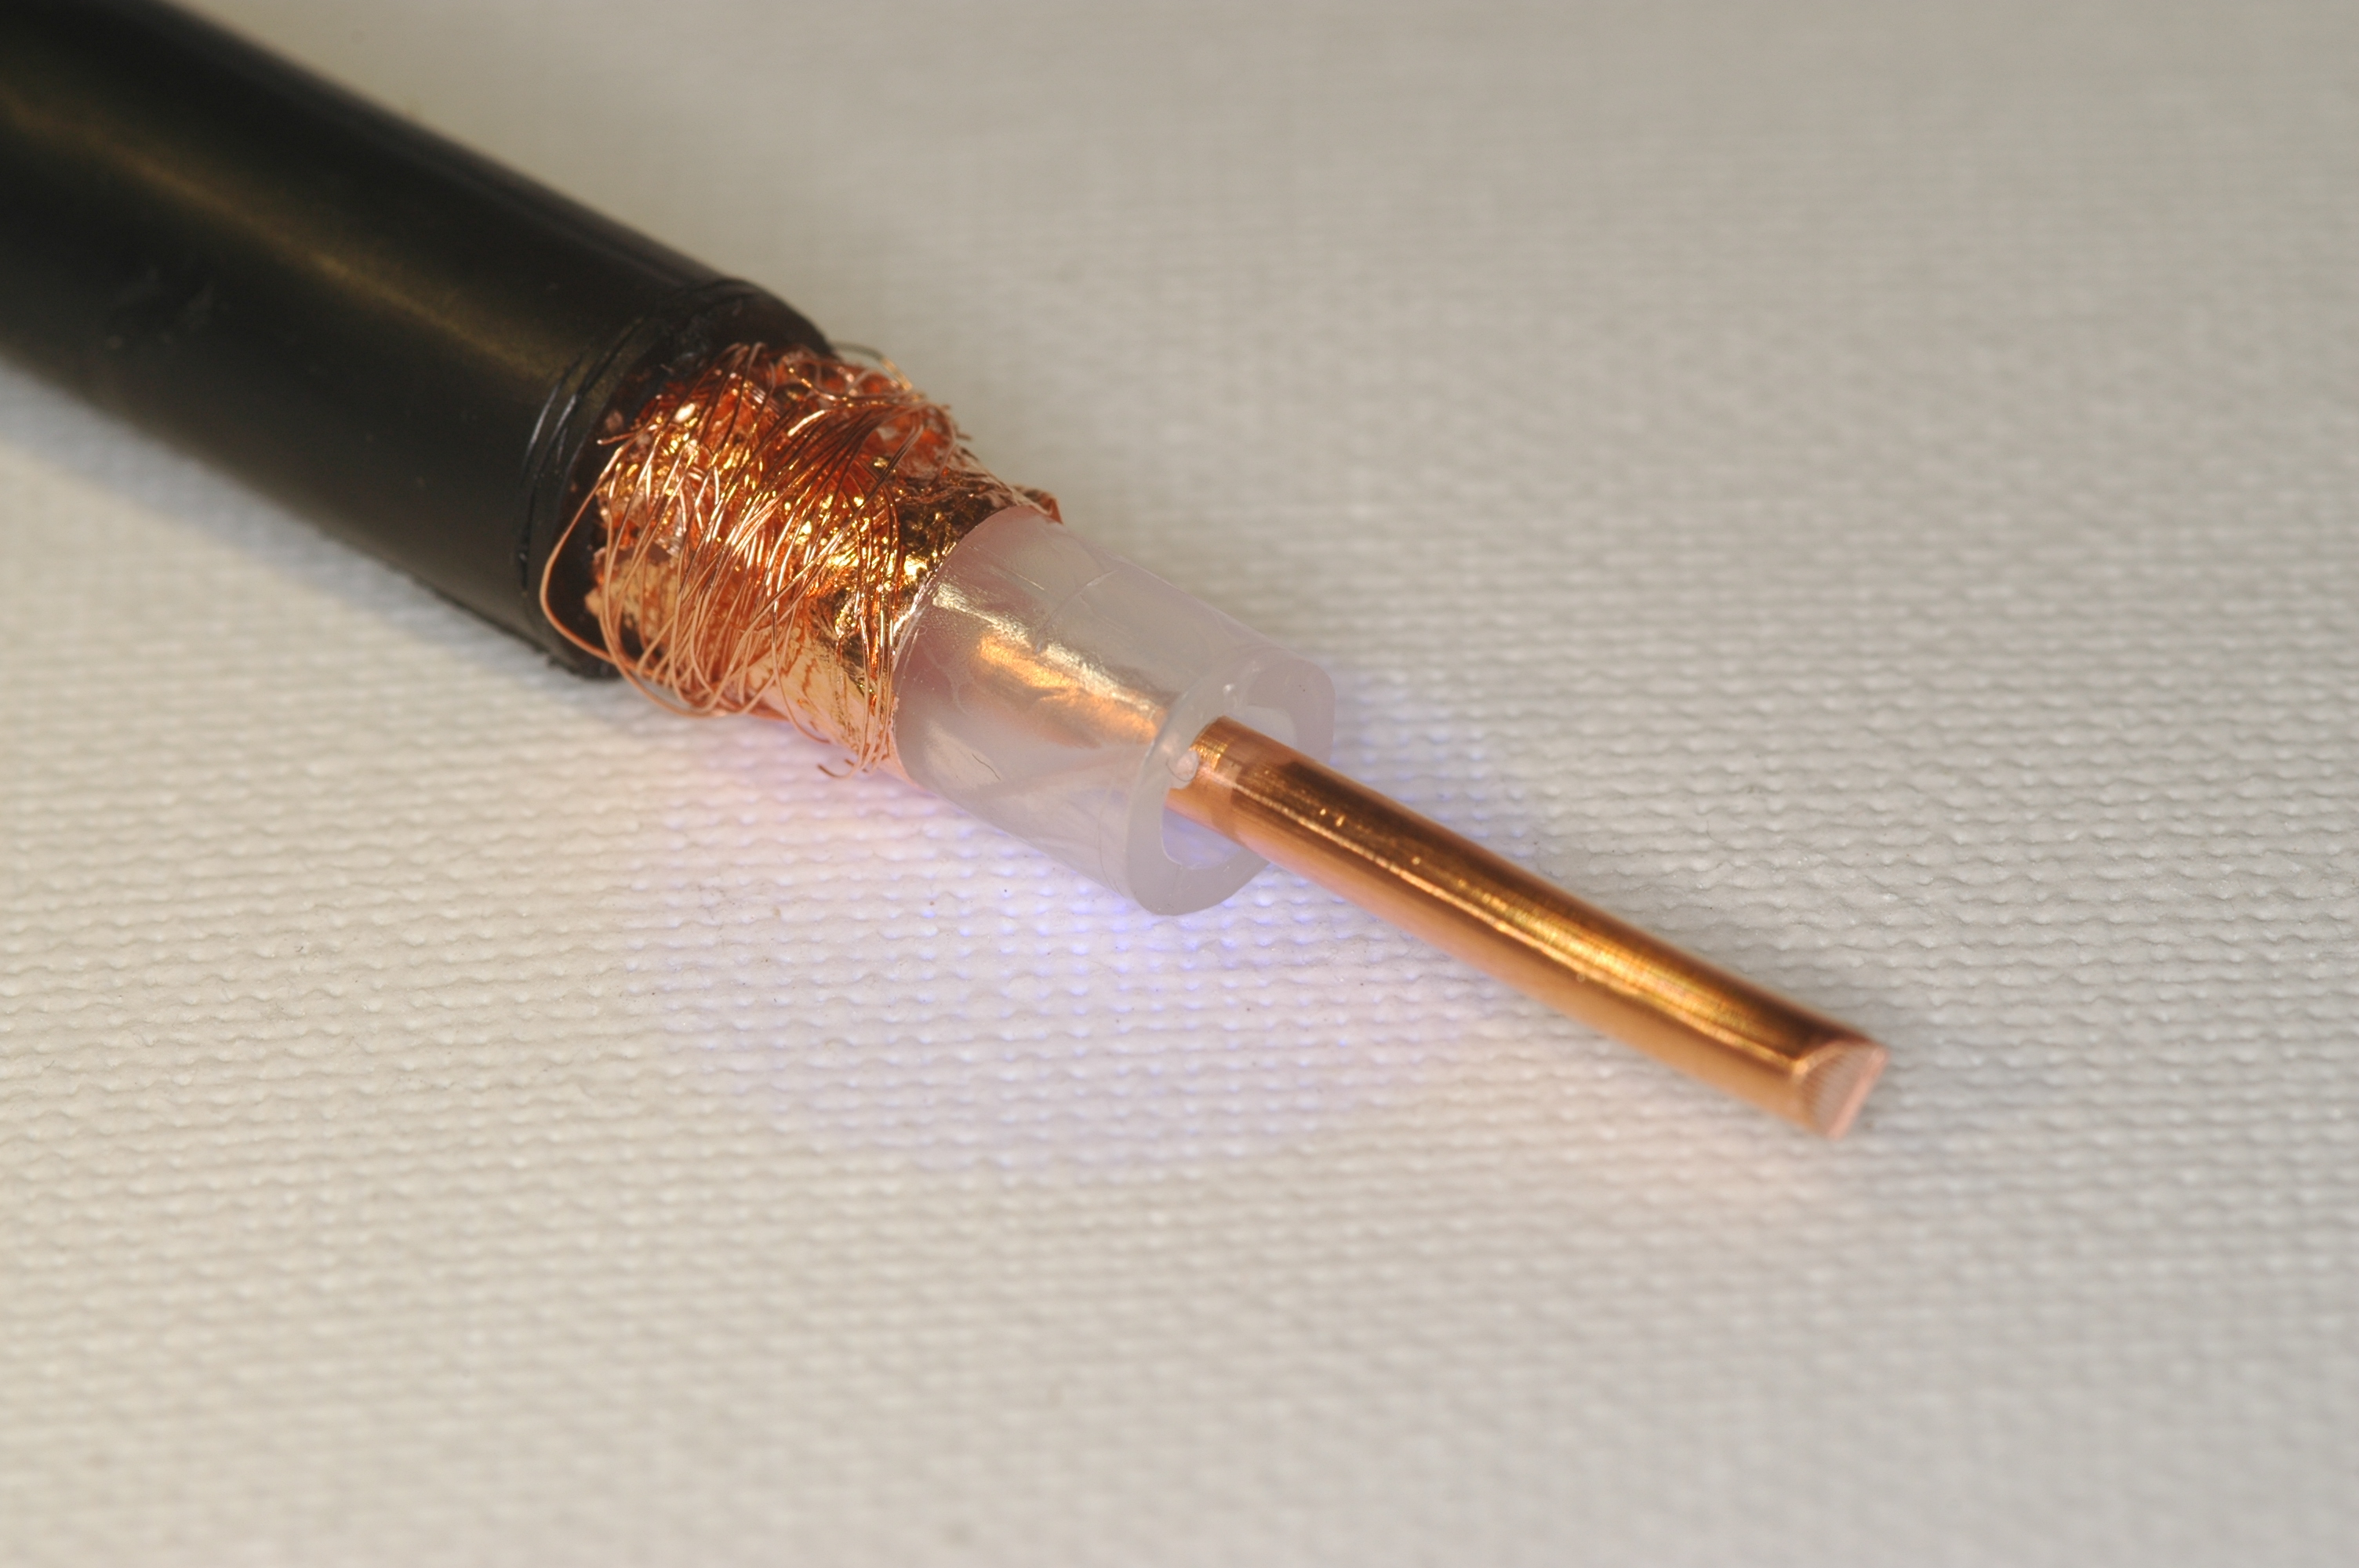
\includegraphics[width=0.85\textwidth]{foto/65}
    \caption{\scriptsize Geöffnetes Koaxialkabel aus Mantel, Schirmung, Dielektrikum und Innenleiter}
    \label{e_uebertragungsleitungen_koaxialkabel}
\end{figure}

    \end{column}
   \begin{column}{0.48\textwidth}
       \begin{itemize}
  \item Wie bei Antennen, ist eine Speiseleitung unsymmetrisch, wenn unterschiedliche Spannungen anliegen
  \item Beim Koaxialkabel sind die beiden Leiter unterschiedlich geformt
  \item Der Schirm weist gegenüber der Erde keine Spannung auf
  \end{itemize}

   \end{column}
\end{columns}

\end{frame}

\begin{frame}
\only<1>{
\begin{QQuestion}{EG304}{Wann ist eine Speiseleitung unsymmetrisch?}{Wenn die Länge nicht einem Vielfachen von $\lambda$/2 entspricht.}
{Wenn die hin- und zurücklaufende Leistung verschieden sind.}
{Wenn sie außerhalb ihrer Resonanzfrequenz betrieben wird.}
{Wenn die beiden Leiter unterschiedlich geformt sind, z. B. Koaxialkabel.}
\end{QQuestion}

}
\only<2>{
\begin{QQuestion}{EG304}{Wann ist eine Speiseleitung unsymmetrisch?}{Wenn die Länge nicht einem Vielfachen von $\lambda$/2 entspricht.}
{Wenn die hin- und zurücklaufende Leistung verschieden sind.}
{Wenn sie außerhalb ihrer Resonanzfrequenz betrieben wird.}
{\textbf{\textcolor{DARCgreen}{Wenn die beiden Leiter unterschiedlich geformt sind, z. B. Koaxialkabel.}}}
\end{QQuestion}

}
\end{frame}

\begin{frame}
\frametitle{Spannungsfestigkeit}
\begin{itemize}
  \item Im Koaxialkabel treten im Dielektrikum Verluste auf
  \item Es kann bei hohen Spannungen zu einem Durchschlag kommen
  \end{itemize}
\end{frame}

\begin{frame}
\only<1>{
\begin{QQuestion}{EG305}{Welche Vorteile hat eine Paralleldraht-Speiseleitung gegenüber der Speisung über ein Koaxialkabel?}{Sie hat geringere Dämpfung und hohe Spannungsfestigkeit.}
{Sie vermeidet Mantelwellen durch Wegfall der Abschirmung.}
{Sie erlaubt leichtere Kontrolle des Wellenwiderstandes durch Verschieben der Spreizer.}
{Sie bietet guten Blitzschutz durch niederohmige Drähte.}
\end{QQuestion}

}
\only<2>{
\begin{QQuestion}{EG305}{Welche Vorteile hat eine Paralleldraht-Speiseleitung gegenüber der Speisung über ein Koaxialkabel?}{\textbf{\textcolor{DARCgreen}{Sie hat geringere Dämpfung und hohe Spannungsfestigkeit.}}}
{Sie vermeidet Mantelwellen durch Wegfall der Abschirmung.}
{Sie erlaubt leichtere Kontrolle des Wellenwiderstandes durch Verschieben der Spreizer.}
{Sie bietet guten Blitzschutz durch niederohmige Drähte.}
\end{QQuestion}

}
\end{frame}

\begin{frame}
\frametitle{Koaxialstecker}
\begin{columns}
    \begin{column}{0.48\textwidth}
    
\begin{figure}
    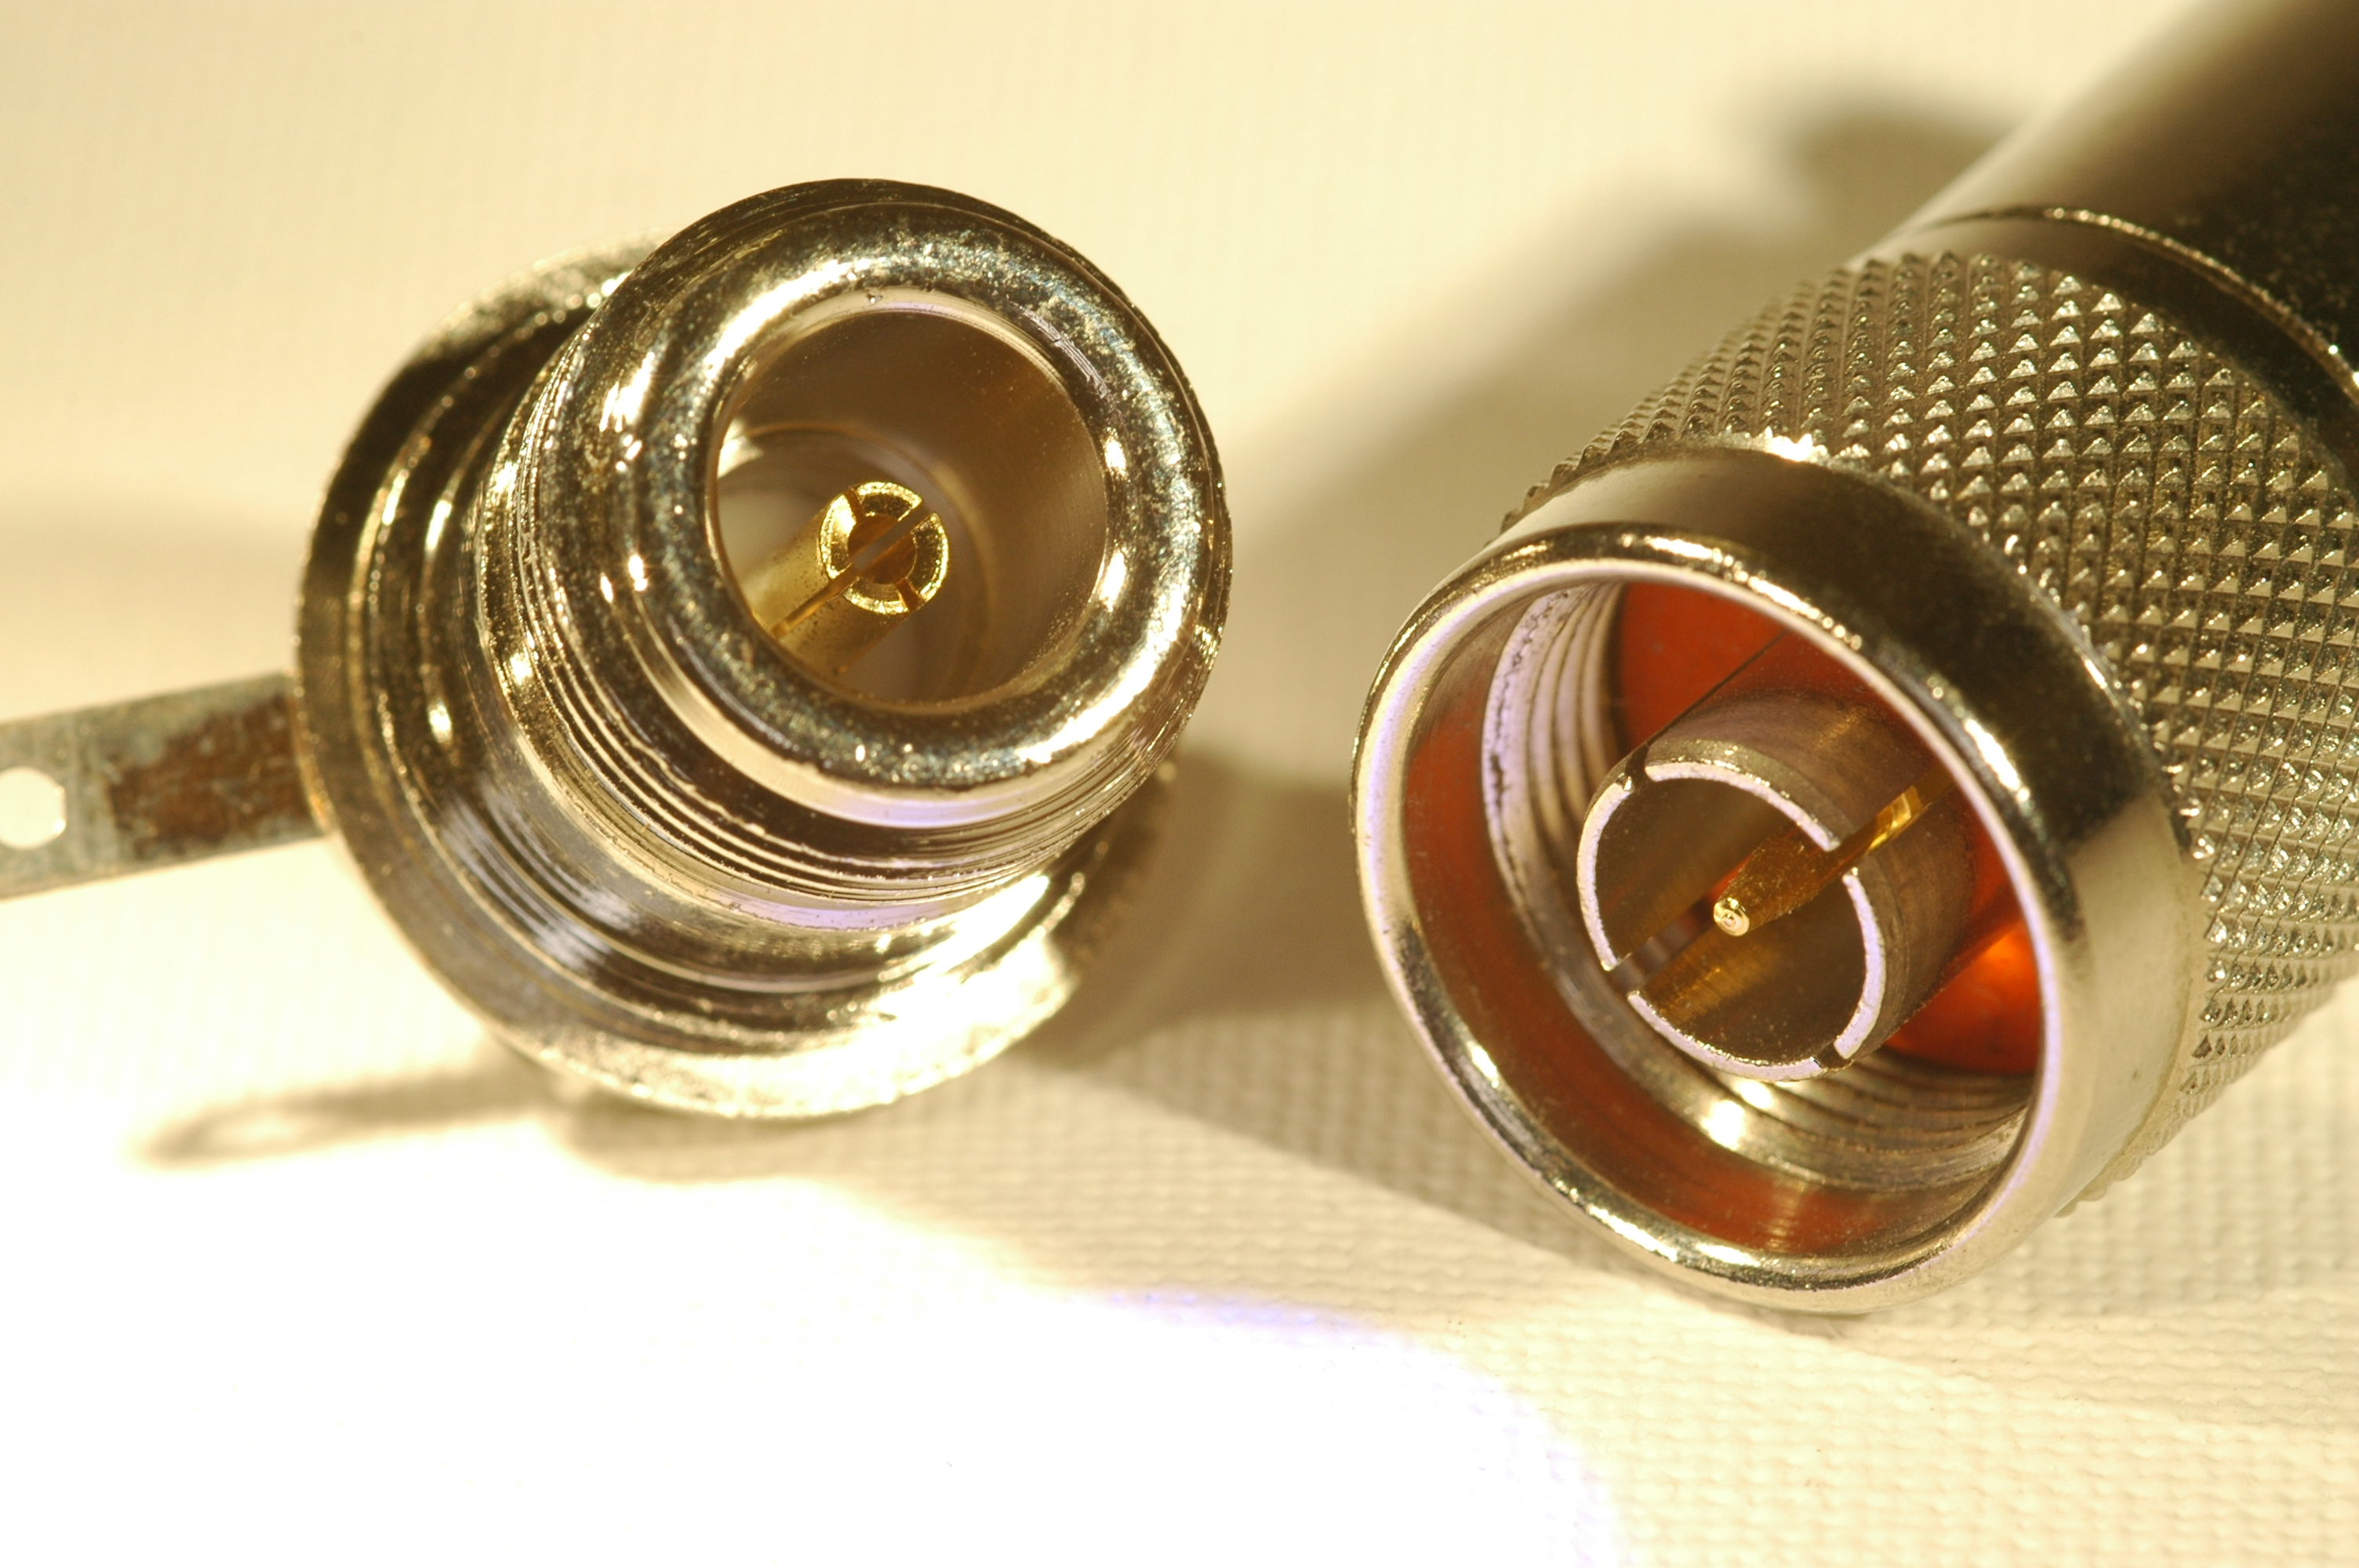
\includegraphics[width=0.85\textwidth]{foto/73}
    \caption{\scriptsize N-Buchse und N-Stecker}
    \label{e_uebertragungsleitungen_n_stecker_buchse}
\end{figure}

    \end{column}
   \begin{column}{0.48\textwidth}
       \begin{itemize}
  \item \emph{N-Stecker}: für niedrige und hohe Frequenz und hohe Leistung
  \item \emph{BNC-Stecker}: für niedrige und hohe Frequenz und geringe Leistung
  \item \emph{SMA-Stecker}: für hohe Frequenz und geringe Leistung
  \item \emph{UHF/PL-Stecker}: für niedrige Frequenz und hohe Leistung
  \end{itemize}

   \end{column}
\end{columns}

\end{frame}

\begin{frame}
\only<1>{
\begin{QQuestion}{EG303}{Welcher der folgenden Koaxialstecker besitzt einen definierten Wellenwiderstand von \qty{50}{\ohm} bis in den GHz-Bereich und hat die höchste Spannungsfestigkeit für die Übertragung hoher Leistungen?}{BNC-Stecker}
{SMA-Stecker}
{UHF-Stecker}
{N-Stecker}
\end{QQuestion}

}
\only<2>{
\begin{QQuestion}{EG303}{Welcher der folgenden Koaxialstecker besitzt einen definierten Wellenwiderstand von \qty{50}{\ohm} bis in den GHz-Bereich und hat die höchste Spannungsfestigkeit für die Übertragung hoher Leistungen?}{BNC-Stecker}
{SMA-Stecker}
{UHF-Stecker}
{\textbf{\textcolor{DARCgreen}{N-Stecker}}}
\end{QQuestion}

}
\end{frame}%ENDCONTENT
